\documentclass{FEIbeamer}

\author[e-mail: cferreira@fei.edu.br]{Prof. Charles Ferreira}

\title{Maratona de Programação FEI}
\subtitle{Ciência da Computação}


\newcommand{\circularpic}[6]{
    \floatnode[x=#1,y=#2]{  
        \begin{tikzpicture}
            \draw[clip] (0,0) ellipse (1.0cm and 1.5cm);
            \node at (#4,#5) {\includegraphics[scale=#6]{#3}};
        \end{tikzpicture}
    }
}
\newcommand{\inlinepic}[2]{
    \raisebox{-10pt}{\tikz{\node{\includegraphics[scale=#2]{#1}};}}
}
\begin{document}

\begin{frame}[fragile]{}
    \question{O que é a Maratona de Programação FEI}
\end{frame}

\begin{frame}[fragile]{Projeto do Curso de Ciência da Computação}
    \textbf{Objetivo:}

    \feibox{Formar equipes para participar de\\ \textgf{Maratonas de Programação}}
    \floatnode[x=6.0,y=1.8]{
\includegraphics[scale=0.15]{imagens/maratona-logo.jpg}}
    \floatnode[x=8.5,y=1.8]{
\includegraphics[scale=0.15]{imagens/maratona_paulista.png}}
    \floatnode[x=3.0,y=1.2]{
\includegraphics[scale=0.4]{imagens/footer_SBC.png}}
    \floatnode[x=13.8,y=0.8]{
\includegraphics[scale=0.15]{imagens/footer_ICPC.jpeg}}
\end{frame}


\begin{frame}[fragile]{Maratona de Programação}

    \bi%
    @ Evento organizado pela sociedade brasileira de computação (SBC)
    @ Estudantes competem para resolver problemas de computação
    \ei%
    \vspace{2cm}

    \floatnode[x=8.0,y=2.5]{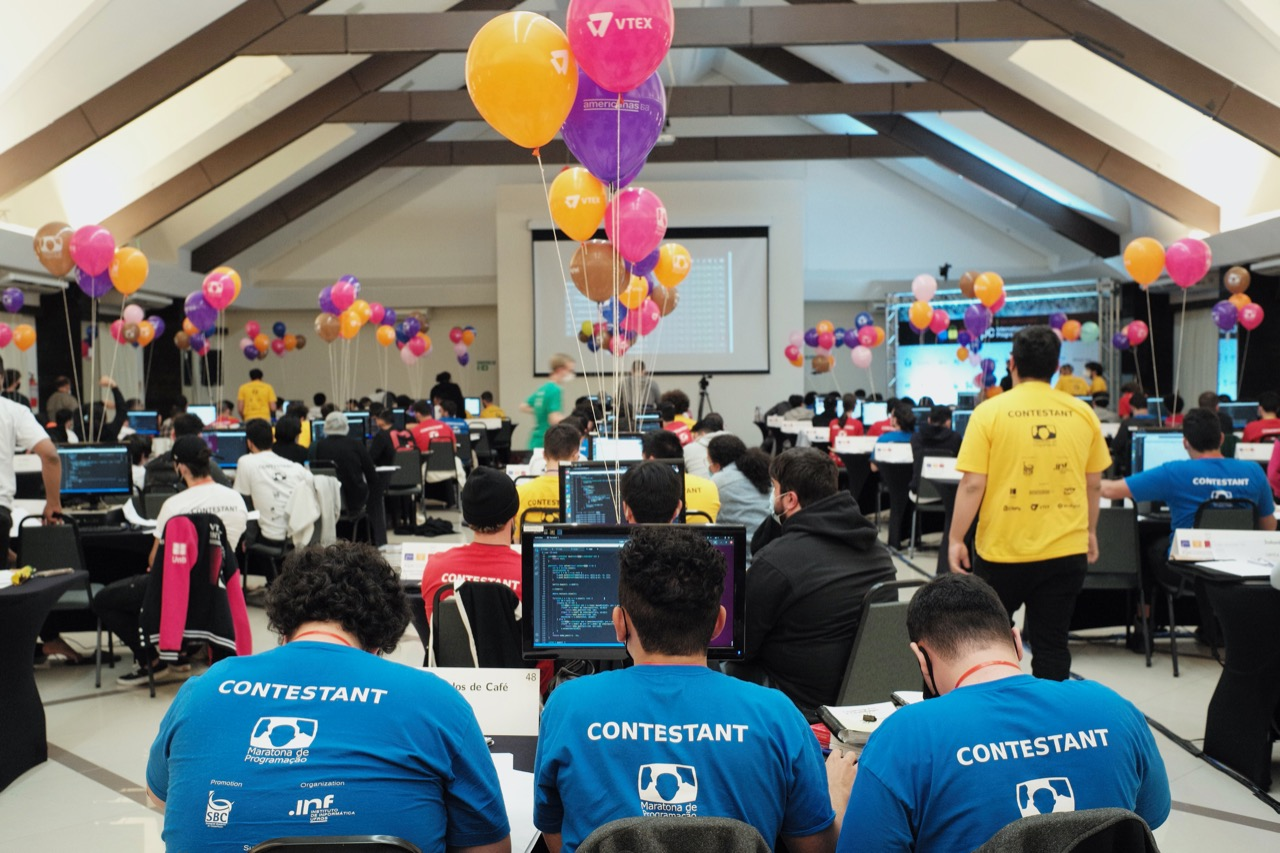
\includegraphics[width=0.90\textwidth,height=0.57\textheight]{imagens/salao21.jpg}}

    \pause\floatnode[x=8,y=2.5]{\feibox{Da maneira mais \textgf{eficiente} possível!}}
    % \grid
\end{frame}

\begin{frame}[fragile]{}
    \question{Qual a vantagem de participar da \textbf{Maratona de Programação}}
\end{frame}

\begin{frame}[fragile]{Vantagens}
    % \grid

    \Activate\doublecolumn[0.6]{%
        % \grid
        \textbf{A competição promove nos estudantes:}\pause
        \bi%
        @ Criatividade \floatnode[x=4.5,y=6.4]{
\includegraphics[scale=0.05]{imagens/idea.png}}\pause
        @ Capacidade de trabalho em equipes\pause
        @ Busca de novas soluções de software\pause
        @ Habilidade de resolver \tikzmarknode[anchor=south east]{pressao}{problemas sob pressão}\pause
        \ei%
        \balloon[follow=pressao,yshift=-1]{Ou seja, o que\\ o mundo real\\ espera de você}
    }{% ---------
        \pause[3]
        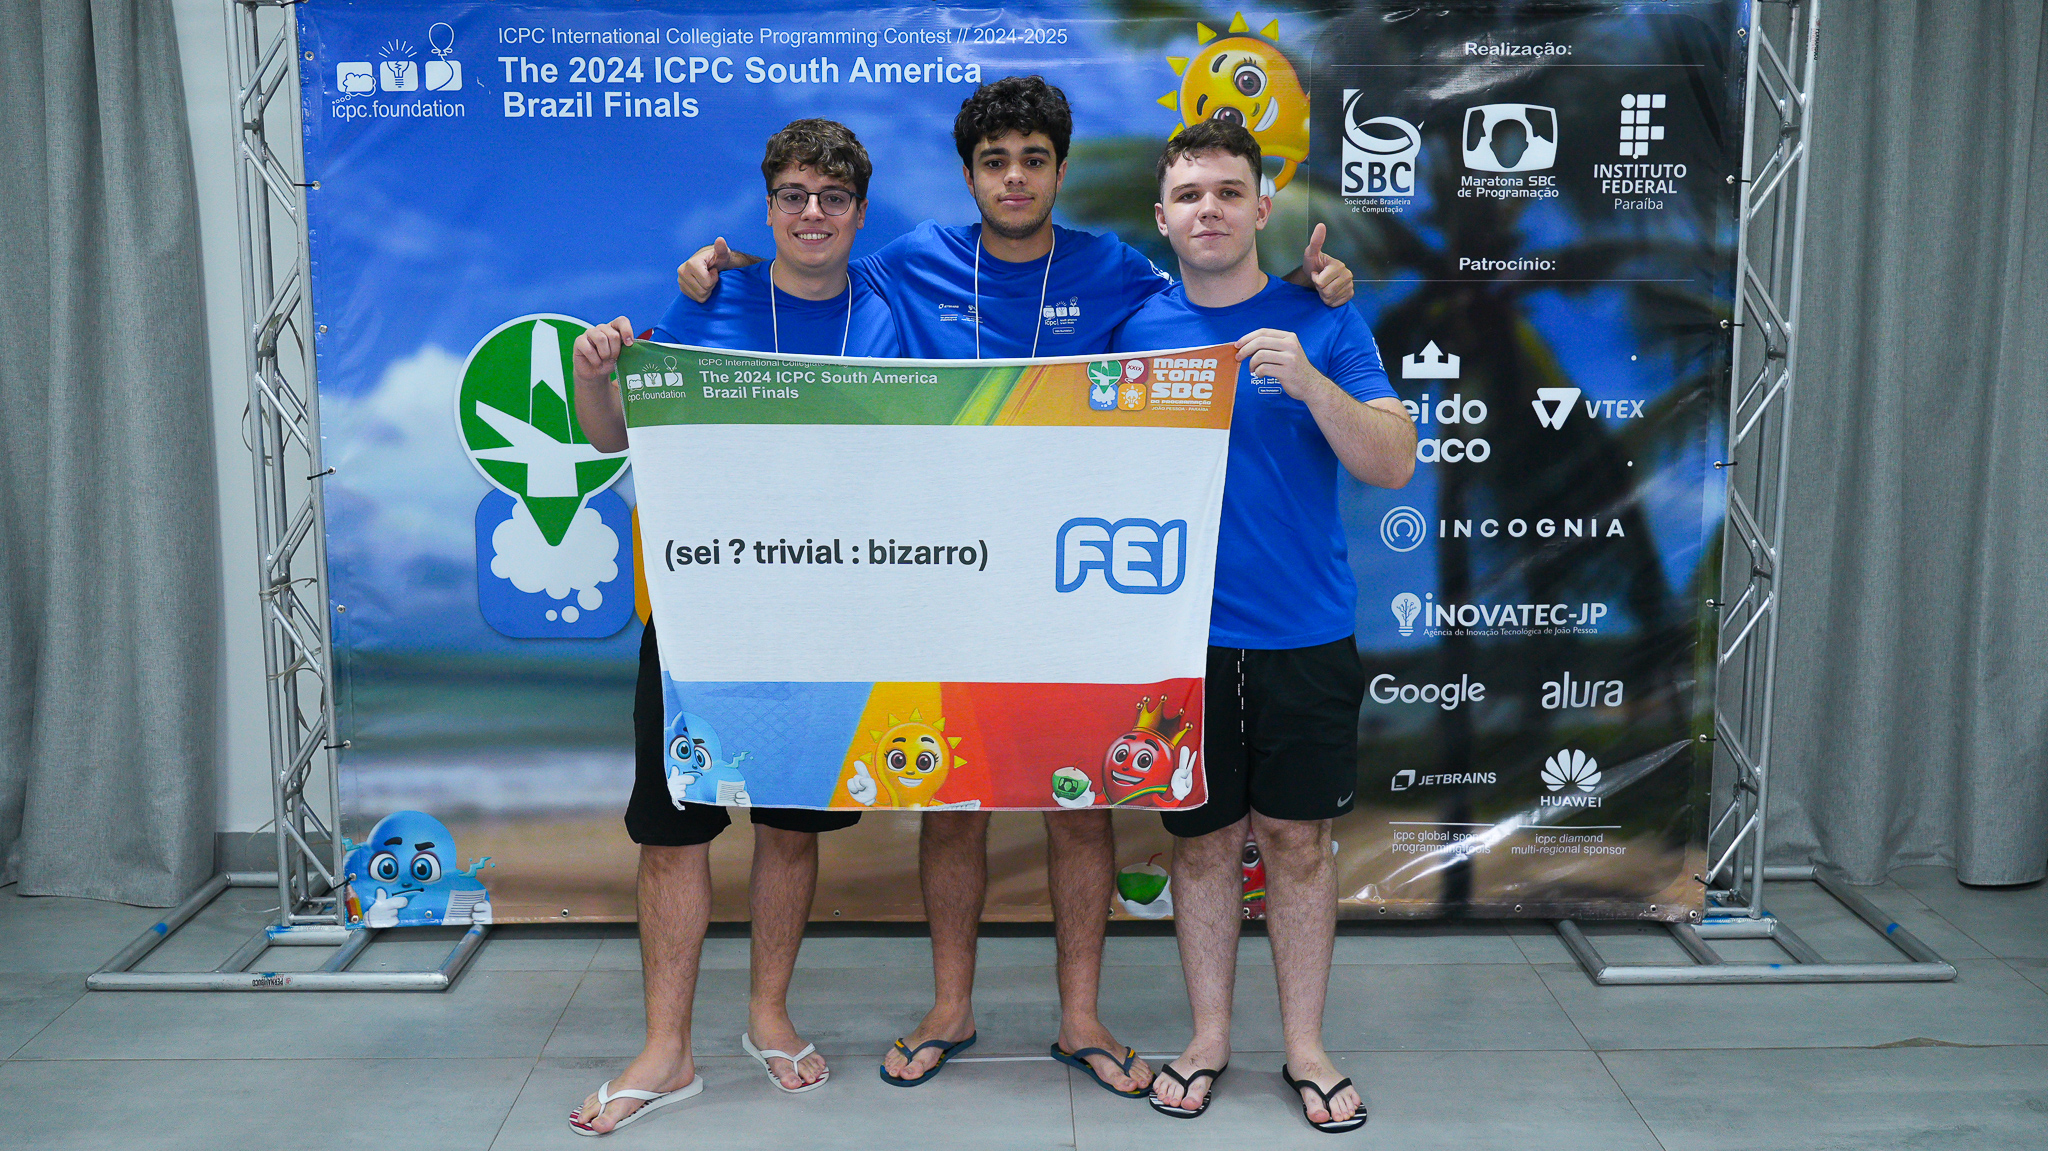
\includegraphics[width=1.0\textwidth,height=0.43\textheight]{imagens/equipe1.jpg}\pause[3]
        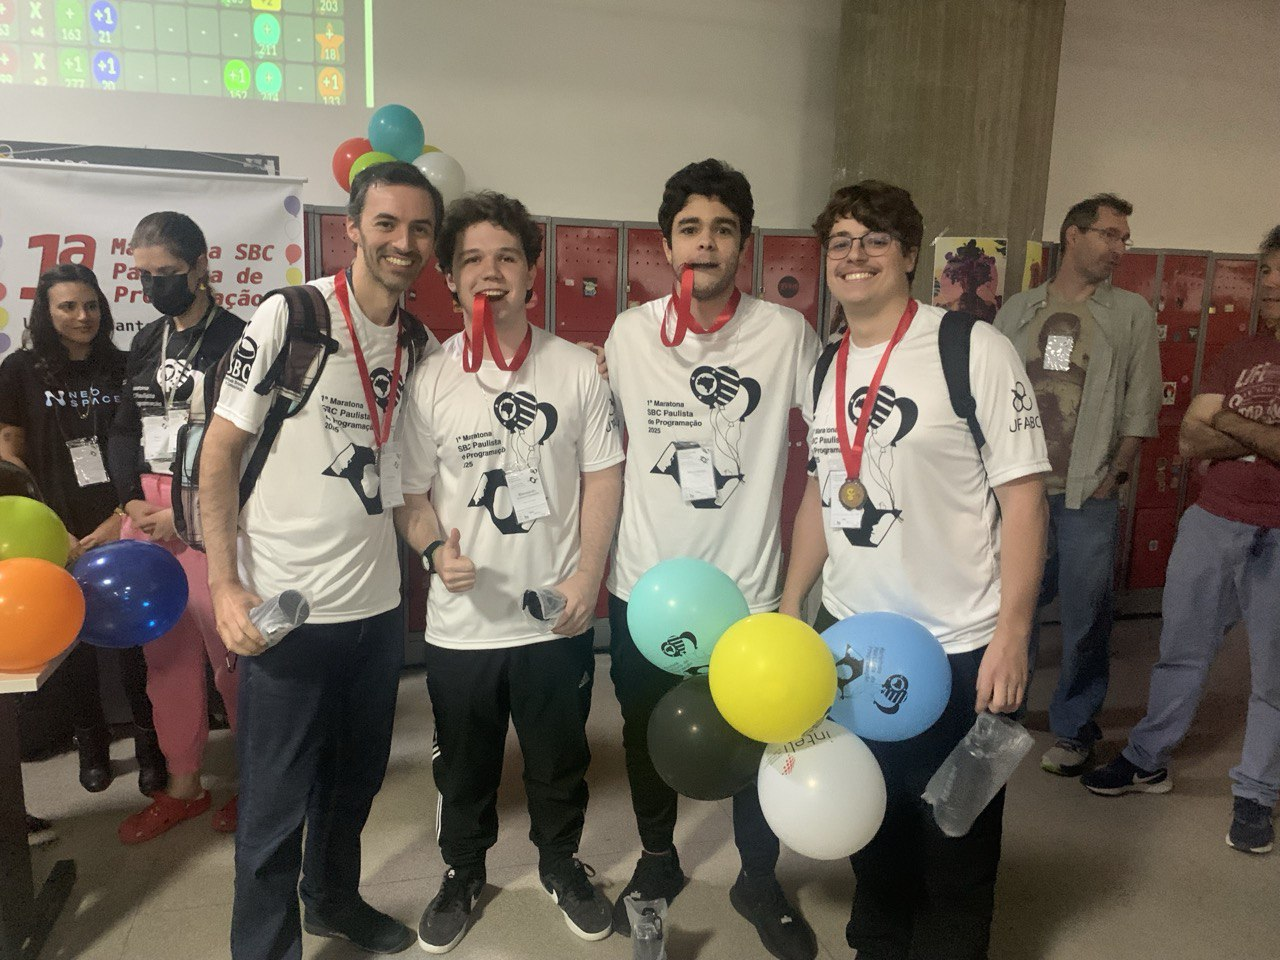
\includegraphics[width=1.0\textwidth,height=0.43\textheight]{imagens/maratona_paulista.jpg}
    }\Deactivate
    % \tiny\url{Photo by <a href="https://unsplash.com/@anniespratt?utm_content=creditCopyText&utm_medium=referral&utm_source=unsplash">Annie Spratt</a> on <a href="https://unsplash.com/photos/group-of-people-using-laptop-computer-QckxruozjRg?utm_content=creditCopyText&utm_medium=referral&utm_source=unsplash">Unsplash</a> }
    % \tiny\url{<a href="https://www.flaticon.com/free-icons/idea" title="idea icons">Idea icons created by Freepik - Flaticon</a>}
\end{frame}

\begin{frame}[fragile]{}
    \Huge
    \centralize{Além disso \ldots}
\end{frame}

\begin{frame}[fragile]{\textcolor{white}{Ambiente de computação}}
    \floatnode[]{
\includegraphics[scale=0.4]{imagens/matrix2.jpg}}
    \color{white}
    \textbf{O aprendizado em computação é enorme!}\pause
    \bi%
    @ Técnicas avançadas de programação e otimização de software\pause
    @ Conceitos de disciplinas dos ciclos finais\pause
    @ Linux, Git, C++, Vim, e muito mais
    \ei%\pause
    % \tiny\url{Foto de <a href="https://unsplash.com/pt-br/@markusspiske?utm_content=creditCopyText&utm_medium=referral&utm_source=unsplash">Markus Spiske</a> na <a href="https://unsplash.com/pt-br/fotografias/filme-matrix-ainda-iar-afB0QQw?utm_content=creditCopyText&utm_medium=referral&utm_source=unsplash">Unsplash</a>}
    \floatnode[x=13.5,y=7.5]{
\includegraphics[scale=0.3]{imagens/tux.png}}
    \floatnode[x=14,y=3.5]{
\includegraphics[scale=0.2]{imagens/c-logo.png}}
    \floatnode[x=11,y=1.5]{
\includegraphics[scale=0.2]{imagens/vim.png}}
    \floatnode[x=6,y=1.5]{
\includegraphics[scale=0.2]{imagens/bash.png}}
    \floatnode[x=2,y=1.5]{
\includegraphics[scale=0.2]{imagens/latex.png}}
    \floatnode[x=5,y=8]{
\includegraphics[scale=0.2]{imagens/git.png}}
\end{frame}


\begin{frame}[fragile]{}
    \question{Quem é a equipe da maratona de programação}
\end{frame}

\begin{frame}[fragile]{Equipe}
    % \grid
    \circularpic{4}{6.0}{imagens/bernardo.jpg}{-2.4}{-2.8}{0.55}
    \circularpic{8}{6.0}{imagens/gabriel.jpeg}{0}{-3.3}{0.3}
    \circularpic{12}{6.0}{imagens/alexandre2.jpg}{-0.4}{-1.3}{0.2}
    \circularpic{4}{2.0}{imagens/GnuFeiCompiler.jpg}{-4.5}{-0.5}{0.35}
    \circularpic{8}{2.0}{imagens/rafael.jpg}{-0.8}{0.8}{0.09}
    \circularpic{12}{2.0}{imagens/GnuFeiCompiler.jpg}{0.20}{-1.0}{0.33}
    \floatnode[x=8,y=8]{\large Gabriel}
    \floatnode[x=4,y=8]{\large Bernardo}
    \floatnode[x=12,y=8]{\large Alexandre}
    \floatnode[x=4,y=4]{\large Luana}
    \floatnode[x=8,y=4]{\large Rafael}
    \floatnode[x=12,y=4]{\large Paulo}
    % \grid
\end{frame}

\begin{frame}[fragile]{}
    \question{Quem está elegível para participar da maratona de programação}
\end{frame}

\begin{frame}[fragile]{Alunos elegíveis}
    \textbf{Todos os alunos:}\pause
    \bi%
    @ Cursando a partir do segundo ciclo\pause
    @ Não tenham DP \pause
    @ Gostem de competição\pause
    @ Tenham disponibilidade de tempo semanal \pause
    @@ no mínimo 3 dias na semana (se puder mais melhor)
    @@ duas horas por dia
    \ei%
\end{frame}

\begin{frame}[fragile]{}
    \question{O que se espera de quem participa da maratona de programação}
\end{frame}

\begin{frame}[fragile]{Programadores da maratona}
    \bi%
    @ Adorem programar!\pause
    @ Queiram aprender muito e compartilhar o que sabem\pause
    @ Tenham auto-motivação e desejem ser auto-didatas
    \ei%
\end{frame}

\begin{frame}[fragile]{}
    \question{O que é preciso fazer para participar da maratona de programação}
\end{frame}

\begin{frame}[fragile]{Como se candidatar}
    \textbf{Os alunos interessados devem se inscrever até 31 de agosto de 2025}

    \feibox{\small Portal do aluno $\to$ sala dos professores $\to$ monitor $\to$ maratona de programação}
    \bi%
    @ Solicitações serão avaliadas; 
    @ Os alunos serão notificados em caso de aceitação
    \ei%
\end{frame}

\begin{frame}[fragile]{}
    \question{Gostaria de conhecer o projeto mas não sei se quero participar. Eu posso}
\end{frame}

\begin{frame}[fragile]{}
    \question{Onde e quando que a equipe se reúne}
\end{frame}

\begin{frame}[fragile]{Encontros}

    \textbf{Sala da Maratona: K409}

        \bi%
        \vspace{-0.5cm}\hrulefill
        @@ Professor: Terça, Quarta e Quinta - 14:00 às 15:00

        \vspace{-0.5cm}\hrulefill
        @@ Segunda - Sexta: 13:00 às 18:00
        @@ Responsáveis: Gabriel e %\inlinepic{example-image-a}{0.1}
        Alexandre %\inlinepic{example-image-a}{0.1} e 

        \vspace{-0.5cm}\hrulefill
        @@ Segunda - Sexta: 09:30 às 12:00
        @@ Responsáveis: Bernardo e %\inlinepic{example-image-a}{0.1} e 
        % Bernardo e %\inlinepic{example-image-a}{0.1}
        Rafael% \inlinepic{example-image-a}{0.1}
        \ei%
    \end{frame}

    \begin{frame}[fragile]{Encontros}
        \textbf{Treinamento semanal}
        \bi%
        @ Os monitores aprimoram suas habilidades nesta sala regularmente.
        @ Compartilham o que sabem.
        @ De tempos em tempos oferecemos aulas práticas de temas correlacionados com a maratona.
        \ei%
    \end{frame}


    \begin{frame}[fragile]{}
        \question{Dúvidas}
    \end{frame}


    \end{document}
